
\documentclass{beamer}
\usetheme[progressbar=frametitle]{metropolis}
\setbeamertemplate{frame numbering}[fraction]
\useoutertheme{metropolis}
\useinnertheme{metropolis}
\usefonttheme{metropolis}
\usecolortheme{spruce}
\setbeamercolor{background canvas}{bg=white}
\usepackage{graphicx} % Allows including images

%----------------------------------------------------------------------------------------
%	TITLE PAGE
%----------------------------------------------------------------------------------------

\definecolor{newgreen}{rgb}{.125,.5,.25}
\usecolortheme[named=newgreen]{structure}

\title[Short title]{The Mathematics of the Rubik's Cube} % The short title appears at the bottom of every slide, the full title is only on the title page

\author{Ellis Pridgeon} % Your name
\institute[University of Bristol] % Your institution as it will appear on the bottom of every slide, may be shorthand to save space
{
University of Bristol \\ % Your institution for the title page
\medskip
\textit{ep15193 - H Level 20CP} % Your email address
}
\date{} % Date, can be changed to a custom date

\begin{document}
\metroset{block=fill}
\begin{frame}
\titlepage % Print the title page as the first slide
\end{frame}

%----------------------------------------------------------------------------------------
%	PRESENTATION SLIDES
%----------------------------------------------------------------------------------------

%------------------------------------------------

\begin{frame}
\frametitle{Composition of the Cube}
\begin{figure}
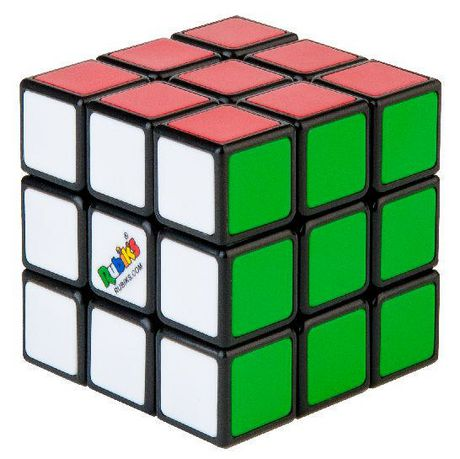
\includegraphics[scale=.5]{rubiks.jpg}
\end{figure}
\begin{itemize}
\item 27 cubes (cubies)
\item 8 corner cubies
\item 12 edge cubies
\item 6 centre cubies
\item One mysterious middle cubie (non visible)
\end{itemize}
\end{frame}

%------------------------------------------------

\begin{frame}
\frametitle{Moves on the Cube}
\begin{figure}
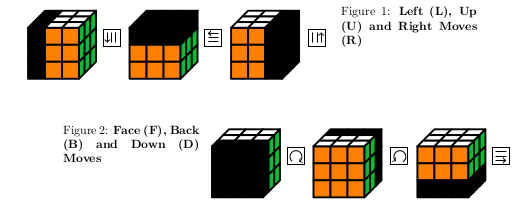
\includegraphics[scale=.5]{rubikmoves.png}
\end{figure}
All moves M – {L,R,U,F,B,D} are permuted by looking at each face and rotating the specific area 90 degress clockwise.

Inverse moves are defined as Lp,Rp,Up which is simply the move in the opposite direction.\\

Also moves L2,R2 denote the move applied twice.
\end{frame}

%------------------------------------------------

\begin{frame}
\frametitle{The Rubik's Cube is a Group}
To prove a group (G,*) is a group under it's operation we must follow the group definition :
\begin{itemize}
\item G is closed under * - So any move applied to the group will still leave the cube in a valid state.
\item G has an identity e – Do nothing
\item G has an inverse – R Rp
\item G is Associative – R (L D) = (R L) D
\end{itemize}
But what is this group ? What is the size ? 
\end{frame}

%------------------------------------------------
\begin{frame}
\frametitle{Size of the group}
Considering the composition:
\begin{align*}
Each\ of\ &the\ 8\ corner\ cubies\ have\ 3\ possible\ faces\\
		&the\ 12\ edge\ cubies\ have\ 2\ possible\ faces\\
		&the\ 6\ center\ cubies\ have\ 1\ possible\ face\\
\end{align*}


$12!\cdot8!\cdot3^8\cdot2^{12}$ $\cong 512$ quintillion different configurations \\
However not all these combinations are possible! This is called the Illegal Cube Group. 
\end{frame}
%------------------------------------------------


\begin{frame}
\frametitle{The Legal Rubik's Cube Group I}
\begin{itemize}
\item To classify the legal group we must make it distinct from all non possible configurations.\\

\item A non possible configuration is one which cant be reached from a set of moves.\\
\end{itemize}

\vspace{3em}
\begin{figure}
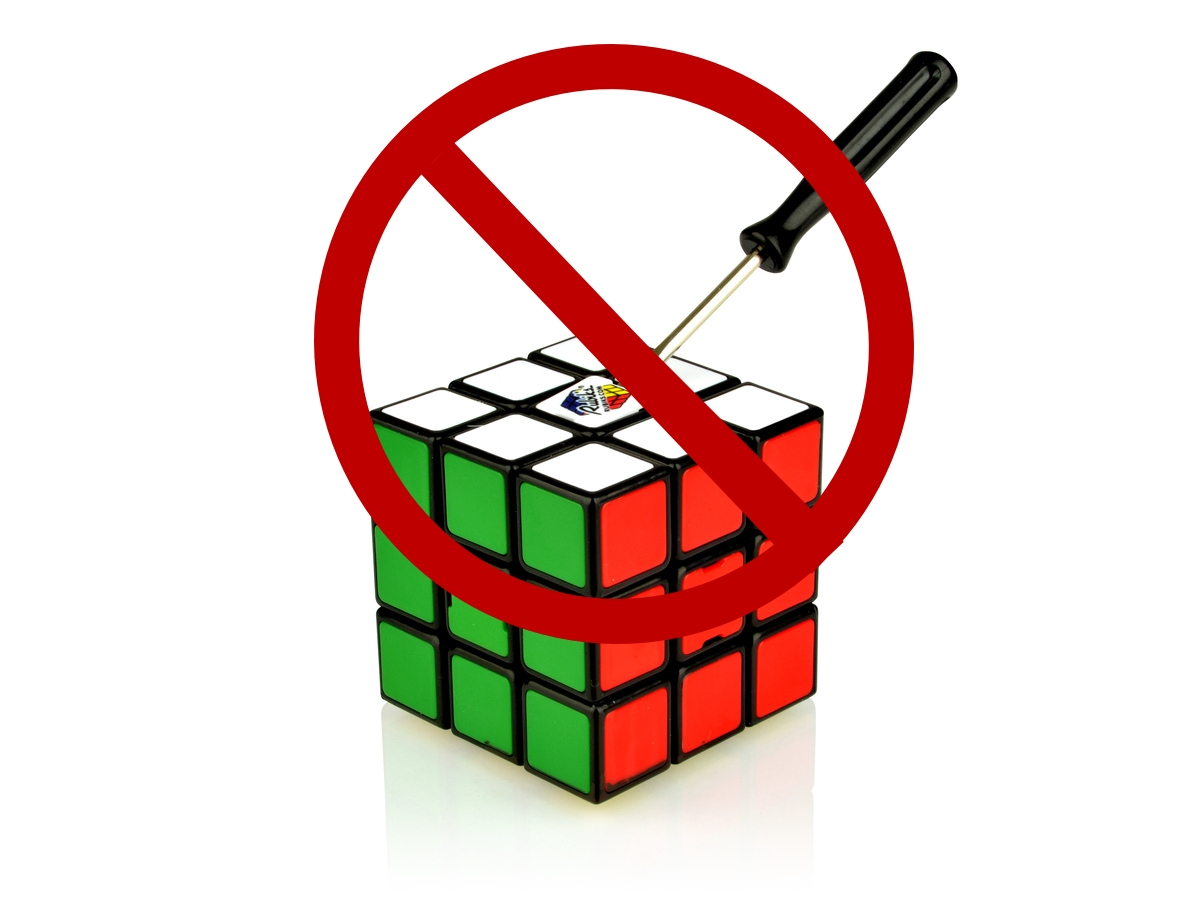
\includegraphics[scale=.1]{no.jpg}
\end{figure}
\end{frame}


%------------------------------------------------

\begin{frame}[t]{The Legal Rubik's Cube Group II}
\begin{block}{Definition: Orbit}
If G acts on a set A, then the orbit of $a \in A$ (under this action) is the set $\{a \cdot g : g \in G\}$ The
stabiliser of an orbit is $\{g \in G|g \cdot x = x\}$ the set of all elements that fix $x$.
\end{block}
\begin{itemize}

\item The legal configurations are configurations which can be found from other possible moves. Moreover, when G acts on the set of cubies the configuration still exists within the orbit set.

\item The solved configuration of the cube is fixed to allow reference to these such moves.
\end{itemize}
\end{frame}

\begin{frame}[t]{A Valid Configuration}
Going back to invalid configurations, we construct a formal definition on what makes these invalid/valid.\\

\begin{center}
$(\tau,\delta,x,y)$
\end{center}
 The x,y values represent the number corresponding to the orientation. While $\tau$ and $\delta$ represent the number of transpositions on $C_{corners}$ and $C_{edges}$.\\
 
We know the group must be made out of some combination of the orientations and permutations. So we can informally classify this group as:\\
\begin{center}
$G_{RC} = C_{Orientations}\ x\ C_{Permutations}$
\end{center}


\end{frame}

\begin{frame}[t]{Orientation Subgroups}
\begin{itemize}

\item Let C be the set of cubies, let G act on C.
\item Consider the two distinct orbits $C_{corners}$ and $C_{edges}$.
\item Firstly consider the subgroup of orientations.
\end{itemize}
\vspace{1em}

\begin{columns}
\column{0.5\textwidth}
\textbf{Corner Cubies}
\begin{itemize}
\item Subgroup - $\mathbb{Z}_3$
\item $\{0,1,2\}$ - 3 different faces
\item Total = $\prod_{i=1}^{7}\mathbb{Z}_3$
\end{itemize}

 
\column{0.5\textwidth}
\textbf{Edge Cubies}
\begin{itemize}
\item Subgroup - $\mathbb{Z}_{2}$
\item $\{0,1\}$ - 2 different faces
\item Total = $\prod_{i=1}^{11} \mathbb{Z}_2$
\end{itemize}
\end{columns}
\begin{center}

The total size of this orientation is simply the direct product between them.
$ \mathbb{Z}_3^8$ X $\mathbb{Z}_2^{12}$, $\ \ \ \ \ $         ($3^7 \cdot 2^{11}$).\\

\end{center}
\end{frame}
%------------------------------------------------


\begin{frame}[t]{The Fundamental Theorem of Cube Theory}
\begin{block}{Theorem: The Fundamental Theorem of Cube Theory}
Let $\tau \in \mathbb{Z}_{3}^{8}$, $\delta \in \mathbb{Z}_{2}^{12}$, x $\in S_{8}$, y $\in S_{12}$ make up a valid configuration $(\tau,\delta, x, y)$ if and only if:
\begin{enumerate}
\item $sgn(\tau) = sgn(\delta)$ (Parity of Permutations)
\item $\Sigma x_{i} =0mod(3)$ (Orientation of Corners)
\item $\Sigma y_{i} =0mod(2)$ (Orientation of Edges)
\end{enumerate}
\end{block}
\end{frame}

\begin{frame}[t]{Semi-direct products}
Next consider the group of permutations, now this is a bit more involved. To do this introduce the idea of a semi-direct product.

\begin{block}{Definition: Semi-Direct Product}
Given group G, subgroup H, normal subgroup N/G and that the following hold.
\begin{itemize}
\item G is the product of subgroups N, H such that G = NH where $N \cap H$ = $e$ the identity
of G
\item There exists a homomorphism $G \rightarrow H$, that is the identity on H whose kernel is N. Then
$G =N \rtimes H$ is a semi-direct product
\end{itemize}
\end{block}
\end{frame}


\begin{frame}[t]{Permutation subgroup}
Again consider the two distinct orbits $C_{corners}$ and $C_{edges}$.
\begin{itemize}
\item By the fundamental theorem of cube theory parity of signs must be equal.
\item By definition an alternating group only contains the even permutations.
\item Thus the direct product contains half $A_8\ x\ A_{12}$  of the total permutations.
\end{itemize}
However this doesn't count any cases where both permutations are odd. It follows that we can take the semi-product of this with $\mathbb{Z}_2$ to obtain the whole subgroup.
\end{frame}

\begin{frame}[t]{The Legal Rubik's Cube Group III}

Thus as the subgroup of permutations is found the legal group can now be defined:

\begin{center}
$G_{RC} = C_{orientations} \rtimes C_{permutaions} = (\mathbb{Z}_2^{12} x \mathbb{Z}_3^8 \rtimes ((A_{8} x A_{12}) \rtimes \mathbb{Z}_2)$
\end{center}
Where $G_{RC}$ has a corresponding size:

\begin{center}
$\frac{1}{2}\cdot 8! \cdot 3^7 \cdot 12! \cdot 2^{11} \cong 43$ quintillion
\end{center}
One twelfth of the original size!
\end{frame}

\begin{frame}[t]{Perfect Efficiency?}
43 quintillion is still a huge amount of configurations.
To achieve perfect efficiency at solving one would need to know the best way to solve the cube from any one of these 43 quintillion. 
\begin{block}{Definition: God's Algorithm}
An algorithm which produces the most optimum solution in the fewest moves. An omniscient being (God) would know all of these optimal steps from any configuration. 
\end{block}

Is this algorithm possible?
\end{frame}

\begin{frame}[t]{History of Efficiency}
\begin{figure}
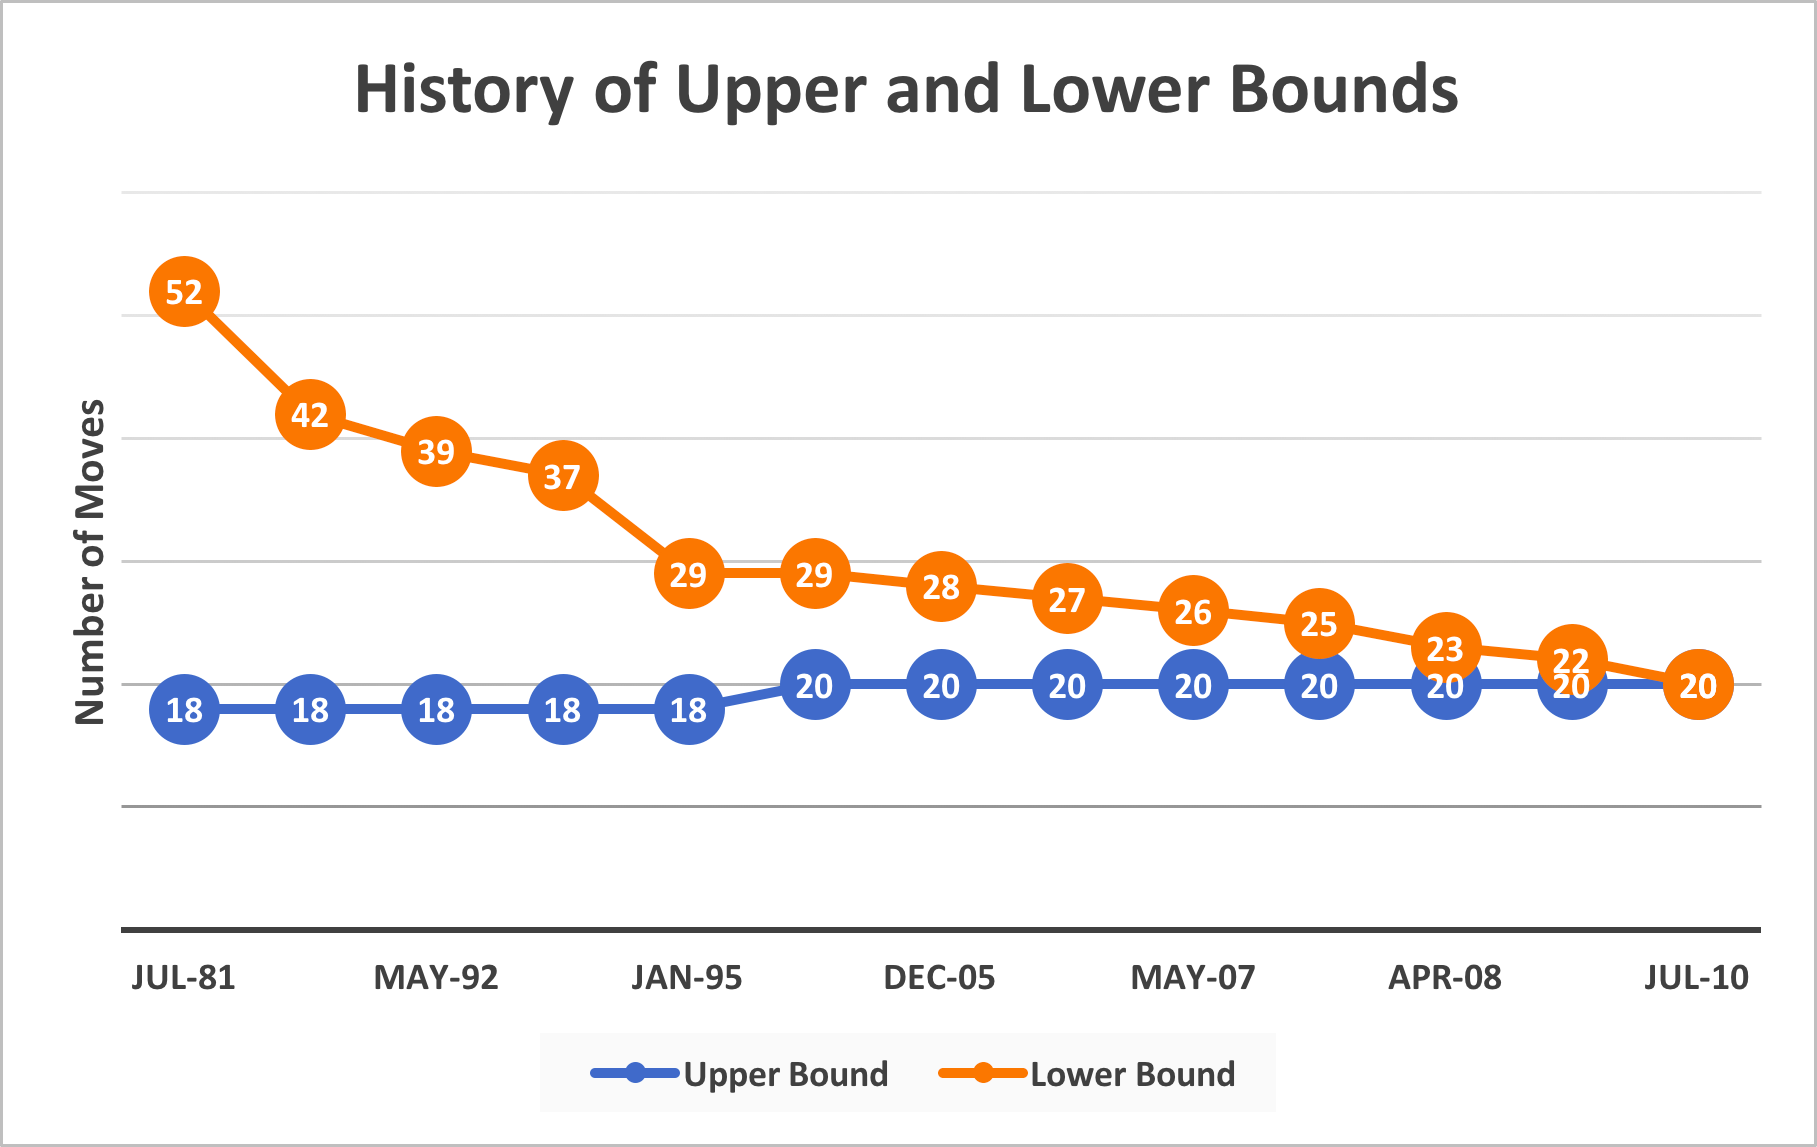
\includegraphics[scale=.15]{historybound.png}
\end{figure}
\end{frame}

\begin{frame}[t]{Technology and the Cube}
\begin{itemize}
\item Optimisations were found by comparing related cosests.
\item This reduced the 43 quintillion valid configurations to 2.2 billion.
\item It took google over 2 weeks to verify this bound of 20 was correct.\end{itemize}
This algorithm though being stepwise efficient is no help when trying to solve the cube in a fast manner.\\

Computationally this in infeasible to implement, as storing all these different configurations becomes an issue.\\

There are many solvers out there where time/efficiency trade offs occur, to allow for the quickest near optimal case possible.
\end{frame}

\begin{frame}[t]{Many Cubes}
The cube is just as popular 30 years from creation\\
Speedcube competitions still occur regularly in the world\\
Motivated the creation of many different variants.

\begin{figure}
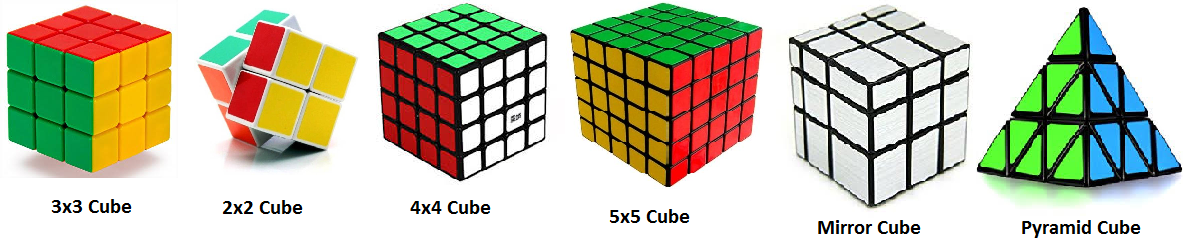
\includegraphics[scale=.3]{diff.png}
\end{figure}
\end{frame}

\begin{frame}[t]{Generators on the groups}
%\vspace{1em}

\begin{columns}
\column{0.5\textwidth}
\textbf{2 by 2}
\begin{itemize}
\item Legal Size -\\  3,674,160
\item Minimal Generators -\\ R,U
\item God's Number - 20
\item World Record = 0.59 seconds
\item 2 generated
\end{itemize}

% \vspace{-1em}
\column{0.5\textwidth}
\textbf{3 by 3}
\begin{itemize}
\item Legal Size -\\  43,252,003,274,489,856,000
\item Minimal Generators -\\ R,L,F,B,U
\item God's Number - 11
\item World Record = 4.59 seconds
\item 2 generated
\end{itemize}
\end{columns}

\begin{align*}
D &= R^{2}L^{2}U^{-1}B^{2}F^{2}U^{-1}B^{2}R^{2}B^{2}F^{2}L^{2}F^{2}U^{-1} \\
D^{-1} &= R^{2}L^{2}UF^{2}B^{2}UF^{2}R^{2}F^{2}B^{2}U^{2}L^{2}U^{2}L^{2}R^{2}U^{2}\\ &R^{2}U^{2}R^{2}F^{2}U^{-1}R^{2}B^{2}R^{2}L^{2}F^{2}L^{2}UB^{2}F^{2}U
\end{align*}
 
\end{frame}


\end{document} 